\begin{figure*}[ht]
\centering
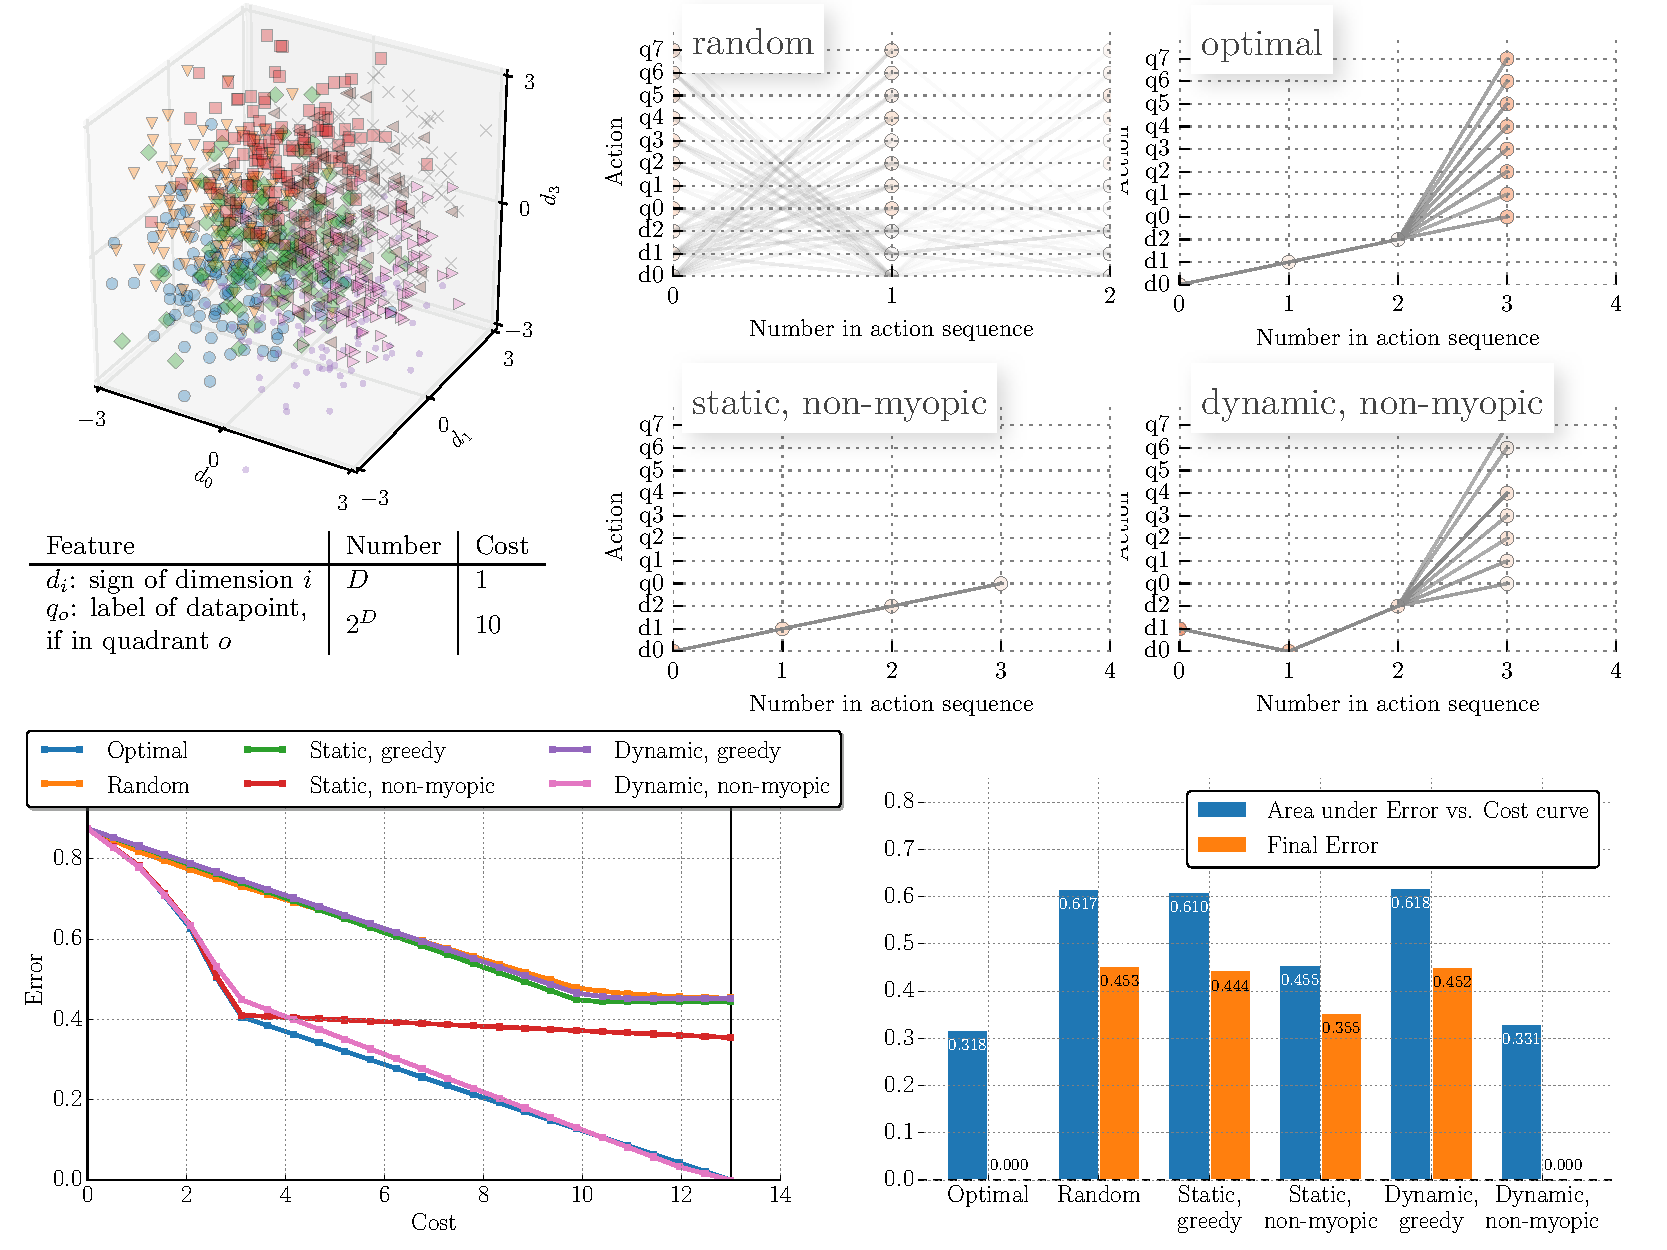
\includegraphics[width=.9\textwidth]{../../figures/synthetic.pdf}
\caption{
Evaluation on the synthetic example (best viewed in color).
The data and the feature costs are shown at top left; the sample feature trajectories of different policies at top right.
(The opacity of the edges corresponds to their prevalence during policy execution; the opacity of the nodes corresponds to the amount of reward obtained in that state.)
Note that the \emph{static, non-myopic} policy correctly learns to select the cheap features first, but is not able to correctly branch, while our \emph{dynamic, non-myopic} approach finds the optimal strategy.
The plots in the bottom half give the error vs. cost numbers.
}\label{fig:synthetic}
\end{figure*}
